\section{问题分析}
\subsection{数据预处理}
数据往往因缺乏统一标准与结构导致杂乱性,因对客观事物在数据库中存在两个以上的描述导致重复性,因信息模糊、随机与缺失导致不完整性。因此为增加模型性能,简化模型计算,我们需要对数据进行预处理。\cite{撇味大白菜2018机器学习笔记:特征工程与数据降维,刘明吉2000数据挖掘中的数据预处理}
\subsubsection{数据清洗}
数据清洗主要包括如下部分:
\begin{enumerate}
    \item\label{P:缺失值} 缺失值处理;
    \item\label{P:噪声} 噪声数据处理;
    \item\label{P:异常值} 异常值处理;
    \item\label{P:脏数据} 脏数据处理;
    \item\label{P:去重} 去重处理。
\end{enumerate}

根据数据集的探索我们可以得出,原数据不存在缺失值,并且结构完善与统一,无重复数据,所以我们只需要进行第~\ref{P:噪声}部分与第~\ref{P:异常值}部分的数据清洗即可。

\subsubsection{数据变换}
数据变换一般包括如下部分\cite{撇味大白菜2018机器学习笔记:特征工程与数据降维}:
\begin{enumerate}
    \item 平滑:去掉数据中的噪音。
    \item 聚集:为多粒度数据分析构造数据。
    \item 数据泛化:用高层次概念代替低层次原始数据。
    \item 规范化:将属性数据按比例缩放,使之落入一个特定区间。
    \item 属性构造:构造新的属性并添加到属性集中。
\end{enumerate}

\subsubsection{数据简化}
数据简化,又称数据规约,指在尽可能保持数据原貌的前提下,最大限度地精简数据量。同时,用于数据简化的时间不应当超过之后在数据挖掘中节省的时间\cite{撇味大白菜2018机器学习笔记:特征工程与数据降维}。数据简化有以下三种常见方法 :
\begin{enumerate}
    \item 维度规约;
    \item 数量规约;
    \item 数据压缩。
\end{enumerate}

本文主要是用维度规约,从高维特征空间向地位特征空间进行映射,即降维。一般来说,现实生活中所得到的数据具备共线性、稀疏性等特征,因此对数据进行降维有助于减少特征属性之间的个数,同时确保特征属性之间是相互独立的。降维主要有以下方法(均来自\verbbox[violet]{sklearn.decomposition}模块)\cite{scikit-learn,sklearn_api,DataAnalyst2019机器学习之sklearn中的降维算法,Cyrille2015sne}:

\begin{itemize}
    \item 主成分分析:
        \begin{itemize}
            \item \verbbox[violet]{PCA};
            \item \verbbox[violet]{IncrementalPCA};
            \item \verbbox[violet]{KernelPCA};
            \item \verbbox[violet]{MiniBatchSparsePCA};
            \item \verbbox[violet]{SparsePCA};
            \item \verbbox[violet]{TruncatedSVD}.
        \end{itemize}
    \item 因子分析:
        \begin{itemize}
            \item \verbbox[violet]{FactorAnalysis}.
        \end{itemize}
    \item 独立成分分析:
        \begin{itemize}
            \item \verbbox[violet]{FastICA}.
        \end{itemize}
    \item 字典学习:
        \begin{itemize}
            \item \verbbox[violet]{DictionaryLearning};
            \item \verbbox[violet]{MiniBatchDictionaryLearning}.
        \end{itemize}
    \item 高级矩阵分解:
        \begin{itemize}
            \item \verbbox[violet]{LatentDirichletAllocation};
            \item \verbbox[violet]{NMF};
            \item \verbbox[violet]{SparseCoder}.
        \end{itemize}
\end{itemize}


\subsection{逻辑斯蒂回归模型构造}
\subsubsection{逻辑斯蒂回归模型}
\begin{theobox}{逻辑斯蒂分布}{logistic-distribution}
    设$X$是连续随机变量,$X$服从逻辑斯蒂分布是指 X具有下列分布函数和密度函数:
        \[
            F(x) = P(X\leq x) = \frac{1}{1+e^{-(x-\mu)/\gamma}}
        \]
        \[
            f(x) = F'(x) = \frac{e^{-(x-\mu)/\gamma}}{\gamma (1+e^{-(x-\mu)/\gamma})^2}
        \]
    式中,$\mu$为位置参数,$\gamma>0$为形状参数。
\end{theobox}

分布函数属于逻辑斯蒂函数,其图像是一条S形曲线(Sigmoid curve)。该曲线以点$(\mu,\tfrac{1}{2})$为中心对称,即满足
\[
    F(-x+\mu)-\frac{1}{2} = -F(x-\mu)+\frac{1}{2}
\]

曲线在中心附近增长速度较快,在两端增长速度较慢,形状参数$\gamma$越小,曲线在中心附近增长得越快。

\subsubsection{二项逻辑斯蒂回归模型}
二项逻辑斯蒂回归模型是一种分类模型,由条件概率分布$P(Y|X)$表示,形式为参数化的逻辑斯蒂分布。这里,随机变量$X$取值为实数,随机变量$Y$取值为1或0.

\begin{theobox}{逻辑斯蒂回归模型}{binomial-logistic-regression-model}
    二项逻辑斯蒂回归模型是如下的条件概率分布:
    \[
        P(Y=1|\vecx) = \frac{\exp(\vecw\cdot\vecx + b)}{1 + \exp(\vecw\cdot\vecx+b)}
    \]
    \[
        P(Y=0|\vecx) = \frac{1}{1 + \exp(\vecw\cdot\vecx+b)}
    \]
    式中,$x\in\RR^n$是输入,$Y\in\{0,1\}$是输出,$w\in\RR^n$ 和$b\in\RR$是参数,$w$称为权值向量,$b$称为偏置,$w\cdot x$为$w$和$x$的内积。
\end{theobox}

对于给定的输入实例$x$,按照定义~\ref{theo:binomial-logistic-regression-model}中的公式可以求得$P(Y=1|x)$和$P(Y=0|x)$,逻辑斯蒂回归比较两个条件概率值的大小,将实例$x$分到概率值较大的那一类。

有时为了方便,将权值向量和输入向量加以扩充,仍记为$\vecw$,$\vecx$,即$\vecw=(w^{(1)},w^{(2)},\ldots,w^{(n)},b)^T$,$\vecx=(x^{(1)},x^{(2)},\ldots,x^{(n)},1)^T$。此时,逻辑斯蒂回归模型如下:
\[
    P(Y=1|\vecx) = \frac{\exp(\vecw\cdot\vecx)}{1+\exp(\vecw\cdot\vecx)}
\]
\[
    P(Y=0|\vecx) = \frac{1}{1+\exp(\vecw\cdot\vecx)}
\]

现在考查逻辑斯蒂回归模型的特点,一个事件的几率(odds)是指该事件发生的概率与该事件不发生的概率的比值,如果事件发生的概率是$p$,那么该事件的几率是$\tfrac{p}{1-p}$,该事件的对数几率(log odds)或$\logit$函数是
\[
    \logit(p) = \log\frac{p}{1-p}
\]

对逻辑斯蒂回归而言,代入可得
\[
    \log\frac{P(Y=1|\vecx)}{1-P(Y=1|\vecx)} = \vecw\cdot\vecx
\]

这就是说,在逻辑斯蒂回归模型中,输出$Y=1$的对数几率是输入$\vecx$的线性函数。或者说,输出$Y=1$的对数几率是由输入$\vecx$的线性函数表示的模型,即逻辑斯蒂回归模型。

\subsubsection{模型参数估计}
逻辑斯蒂回归模型学习时,对于给定的训练数据集$T=\{(\vecx_1,y_1),(\vecx_2,y_2),\ldots,(\vecx_N,y_N)\}$,其中$\vecx_i\in\RR^n$,$y_i\in\{0,1\}$,可以应用极大似然估计法估计模型参数,从而得到逻辑斯蒂回归模型。

设$P(Y=1|\vecx)=\pi(\vecx)$,$P(Y=0|\vecx)=1-\pi(\vecx)$,似然函数为
\[
    \prod_{i=1}^N[\pi(\vecx_i)]^{y_i}[1-\pi(\vecx_i)]^{1-y_i},
\]
对数似然函数为
\[
    \begin{aligned}
        L(\vecw) &= \sum_{i=1}^N[y_i\log\pi(\vecx_i)+(1-y_i)\log(1-\pi(\vecx_i))] \\
                 &= \sum_{i=1}^N\left[y_i\log\frac{\pi(\vecx_i)}{1-\pi(\vecx_i)}+\log(1-\pi(\vecx_i))\right] \\
                 &= \sum_{i=1}^N[y_i(\vecw\cdot\vecx_i)-\log(1+\exp(\vecw\cdot\vecx_i))]
    \end{aligned}
\]

对$L(\vecw)$求极大值,得到$\vecw$的估计值。这样,问题就变成了以对数似然函数为目标函数的最优化问题。逻辑斯蒂回归学习中通常采用的办法是梯度下降法及拟牛顿法。

假设$\vecw$的极大似然估计值是$\hat\vecw$,那么学到的逻辑斯蒂回归模型为
\[
    P(Y=1|\vecx) = \frac{\exp(\hat\vecw\cdot\vecx)}{1+\exp(\hat\vecw\cdot\vecx)}
\]
\[
    P(Y=0|\vecx) = \frac{1}{1+\exp(\hat\vecw\cdot\vecx)}
\]


\subsection{其他回归模型构造}
\subsubsection{评价与误差函数}
我们选择以下评价函数与误差函数来评定模型的优劣(均来自于\verbbox[violet]{sklearn.metrics}模块):
\begin{itemize}
    \item 评价函数:
        \begin{itemize}
            \item \verbbox[violet]{explained_variance_score};
            \item \verbbox[violet]{r2_score}.
        \end{itemize}
    \item 误差函数:
        \begin{itemize}
            \item \verbbox[violet]{max_error};
            \item \verbbox[violet]{mean_absolute_error};
            \item \verbbox[violet]{mean_squared_error};
            \item \verbbox[violet]{mean_squared_log_error};
            \item \verbbox[violet]{median_absolute_error}.
        \end{itemize}
\end{itemize}

广泛地对模型进行评价,同时加上模型的训练时间与预测时间,多维度地评价模型的优劣。

\subsubsection{回归模型的选择}
广泛地训练模型,从而取效果最好的,因此我们采用以下的回归模型\cite{scikit-learn,sklearn_api}:
\begin{itemize}
    \item \verbbox[violet]{sklearn.ensemble}:
        \begin{itemize}
            \item \verbbox[violet]{AdaBoostRegressor};
            \item \verbbox[violet]{BaggingRegressor};
            \item \verbbox[violet]{ExtraTreesRegressor};
            \item \verbbox[violet]{GradientBoostingRegressor};
            \item \verbbox[violet]{IsolationForest}.
        \end{itemize}
    \item \verbbox[violet]{sklearn.gaussian_process}:
        \begin{itemize}
            \item \verbbox[violet]{GaussianProcessRegressor}.
        \end{itemize}
    \item \verbbox[violet]{sklearn.linear_model}:
        \begin{itemize}
            \item \verbbox[violet]{ElasticNetCV};
            \item \verbbox[violet]{HuberRegressor};
            \item \verbbox[violet]{LassoLarsCV};
            \item \verbbox[violet]{LogisticRegression};
            \item \verbbox[violet]{PassiveAggressiveRegressor};
            \item \verbbox[violet]{RANSACRegressor};
            \item \verbbox[violet]{RidgeCV};
            \item \verbbox[violet]{SGDRegressor};
            \item \verbbox[violet]{TheilSenRegressor}.
        \end{itemize}
    \item \verbbox[violet]{sklearn.neighbors}:
        \begin{itemize}
            \item \verbbox[violet]{KNeighborsRegressor};
            \item \verbbox[violet]{RadiusNeighborsRegressor}.
        \end{itemize}
    \item \verbbox[violet]{sklearn.neural_network}:
        \begin{itemize}
            \item \verbbox[violet]{MLPRegressor}.
        \end{itemize}
\end{itemize}

最后生成一个数据结构如下的结果:

\tikz [font=\texttt\footnotesize,
    grow=right, level 1/.style={sibling distance=3em,level distance=.1\textwidth},
                level 2/.style={sibling distance=3em,level distance=.15\textwidth},
                level 3/.style={sibling distance=1.5em,level distance=.2\textwidth},
                level 4/.style={sibling distance=1em,level distance=.25\textwidth},]
    \node{Result}
        child { node{cnt}
            child { node{\dots} }
        }
        child { node{casual}
            child { node{\dots} }
        }
        child { node{registered}
            child { node{info}
                child { node{\vdots} }
                child { node{AdaBoostRegressor}
                    child { node{r2\_score} }
                    child { node{fit\_time} }
                    child { node{pred\_time} }
                }
            }
            child { node{best}
                child { node{model} }
                child { node{r2\_score} }
            }
        };


\subsection{数据可视化示例}
\subsubsection{数据探索}
数据集见问题描述章节真实数据描述小节。

首先我们将数据集分为训练集与测试集,以此判断回归模型的好坏与避免模型的欠拟合与过拟合。按照规则,我们提取出每月前19天作为训练集,其余天数作为测试集。将除\verbbox[blue]{casual}、\verbbox[blue]{registered}与\verbbox[blue]{cnt}这三列的数据视做变量向量$\vecx$,将\verbbox[blue]{cnt}列视做响应向量$\vecy$。

其次我们计算出数据的描述性统计量,以此大致判断数据集的分布及形状。由表~\ref{T:train-day_x-data}、表与\ref{T:train-day_y-data}可以得出训练集的个数、均值、方差、最小最大值与分位数。部分列向量已经过归一化处理,不难看出数据基本不符合正态分布,同时由\verbbox[violet]{scipy.stats.kstest}计算可得出上述结论。

\begin{table}[htbp]
    \centering\tiny
    \begin{tabular}{lrrrrrrrrrrr}
    \toprule
    {} &  season &     yr &    mnth &  holiday &  weekday &  workingday &  weathersit &    temp &   atemp &     hum &  windspeed \\
    \midrule
    count &  456 &  -  &   -  &   -  &   -  &   -  &   -  &   -  &   -  &   -  &   -  \\
    mean  & 2.50 & 0.5 & 6.50 & 0.03 & 3.00 & 0.68 & 1.39 & 0.49 & 0.47 & 0.62 & 0.19 \\
    std   & 1.12 & 0.5 & 3.46 & 0.17 & 2.01 & 0.47 & 0.54 & 0.18 & 0.16 & 0.14 & 0.08 \\
    min   & 1.00 & 0.0 & 1.00 & 0.00 & 0.00 & 0.00 & 1.00 & 0.11 & 0.10 & 0.00 & 0.02 \\
    25\%  & 1.75 & 0.0 & 3.75 & 0.00 & 1.00 & 0.00 & 1.00 & 0.34 & 0.34 & 0.51 & 0.14 \\
    50\%  & 2.50 & 0.5 & 6.50 & 0.00 & 3.00 & 1.00 & 1.00 & 0.50 & 0.49 & 0.62 & 0.18 \\
    75\%  & 3.25 & 1.0 & 9.25 & 0.00 & 5.00 & 1.00 & 2.00 & 0.65 & 0.60 & 0.72 & 0.23 \\
    max   & 4.00 & 1.0 &12.00 & 1.00 & 6.00 & 1.00 & 3.00 & 0.86 & 0.80 & 0.97 & 0.51 \\
    \bottomrule
    \end{tabular}
    \cprotect\caption{\verbbox[gray]{day.csv}训练集变量数据探索}\label{T:train-day_x-data}
\end{table}

\begin{table}[htbp]
    \centering\tiny
    \begin{tabular}{lrrr}
    \toprule
    {}    &  casual & registered &  cnt \\
    \midrule
    count &    456  &     -   &     -   \\
    mean  &  859.95 & 3713.47 & 4573.41 \\
    std   &  698.91 & 1494.48 & 1868.74 \\
    min   &    9.00 &  491.00 &  605.00 \\
    25\%  &  318.00 & 2696.00 & 3305.50 \\
    50\%  &  722.00 & 3700.00 & 4585.50 \\
    75\%  & 1141.75 & 4814.25 & 5987.50 \\
    max   & 3410.00 & 6911.00 & 8714.00 \\
    \bottomrule
    \end{tabular}
    \cprotect\caption{\verbbox[gray]{day.csv}训练集相应数据探索}\label{T:train-day_y-data}
\end{table}

\begin{table}[htbp]
    \centering\tiny
    \begin{tabular}{lrrrrrrrrrrrr}
    \toprule
    {}    & season & yr &  mnth & hr & holiday & weekday & workingday & weathersit & temp & atemp & hum & windspeed \\
    \midrule
    count & 10886 &  -  &   -   &    -  &   -  &   -  &   -  &   -  &   -  &   -  &   -  &   -  \\
    mean  &  2.51 & 0.5 &  6.52 & 11.54 & 0.03 & 3.00 & 0.68 & 1.42 & 0.49 & 0.47 & 0.62 & 0.19 \\
    std   &  1.12 & 0.5 &  3.44 &  6.92 & 0.17 & 2.01 & 0.47 & 0.63 & 0.19 & 0.17 & 0.19 & 0.12 \\
    min   &  1.00 & 0.0 &  1.00 &  0.00 & 0.00 & 0.00 & 0.00 & 1.00 & 0.02 & 0.02 & 0.00 & 0.00 \\
    25\%  &  2.00 & 0.0 &  4.00 &  6.00 & 0.00 & 1.00 & 0.00 & 1.00 & 0.34 & 0.33 & 0.47 & 0.10 \\
    50\%  &  3.00 & 1.0 &  7.00 & 12.00 & 0.00 & 3.00 & 1.00 & 1.00 & 0.50 & 0.48 & 0.62 & 0.19 \\
    75\%  &  4.00 & 1.0 & 10.00 & 18.00 & 0.00 & 5.00 & 1.00 & 2.00 & 0.64 & 0.62 & 0.77 & 0.25 \\
    max   &  4.00 & 1.0 & 12.00 & 23.00 & 1.00 & 6.00 & 1.00 & 4.00 & 1.00 & 0.91 & 1.00 & 0.85 \\
    \bottomrule
    \end{tabular}
    \cprotect\caption{\verbbox[gray]{hour.csv}训练集变量数据探索}\label{T:train-hour_x-data}
\end{table}

\begin{table}[htbp]
    \centering\tiny
    \begin{tabular}{lrrr}
    \toprule
    {}    & casual & registered & cnt \\
    \midrule
    count &  10886 &    -   &    -    \\
    mean  &  36.02 & 155.55 & 191.57  \\
    std   &  49.96 & 151.04 & 181.14  \\
    min   &   0.00 &   0.00 &   1.00  \\
    25\%  &   4.00 &  36.00 &  42.00  \\
    50\%  &  17.00 & 118.00 & 145.00  \\
    75\%  &  49.00 & 222.00 & 284.00  \\
    max   & 367.00 & 886.00 & 977.00  \\
    \bottomrule
    \end{tabular}
    \cprotect\caption{\verbbox[gray]{hour.csv}训练集相应数据探索}\label{T:train-hour_y-data}
\end{table}

\subsubsection{数据可视化}
接下来我们对数据进行可视化处理,以期得到更加直观的结论,并且简要验证上述的假设。数据由两个数据集构成,我们分别将数据集分为训练集与测试集,同时衍生出时间相关变量数据集。

如图~\ref{F:train-day},\verbbox[gray]{day.csv}训练集中响应(注册用户数目、未注册用户数目与总用户数目)趋势基本一致,并且与温度、体感温度的趋势趋于一致,而湿度与风速则直观感觉不到相似的趋势。

如图~\ref{F:train-hour},\verbbox[gray]{hour.csv}训练集的可视化中记录了一周内24小时的用户数量。可以看出响应(注册用户数目、未注册用户数目与总用户数目)趋势基本一致,类似于周期函数,且一共有14个峰值,分别出现在早高峰与晚高峰时段,而工作日(周一至周五)的用户数量是多于周末(周六与周日)的。直观来说,不同时间段用户数量与温度、体感温度、湿度、风速均有一定的联系,不好判断哪一个变量为主要变量,于是就需要训练回归模型预测。
\begin{figure}[htbp]
    \centering
    \cprotect\subcaptionbox{\verbbox[gray]{day.csv}训练集数据可视化\label{F:train-day}}
        {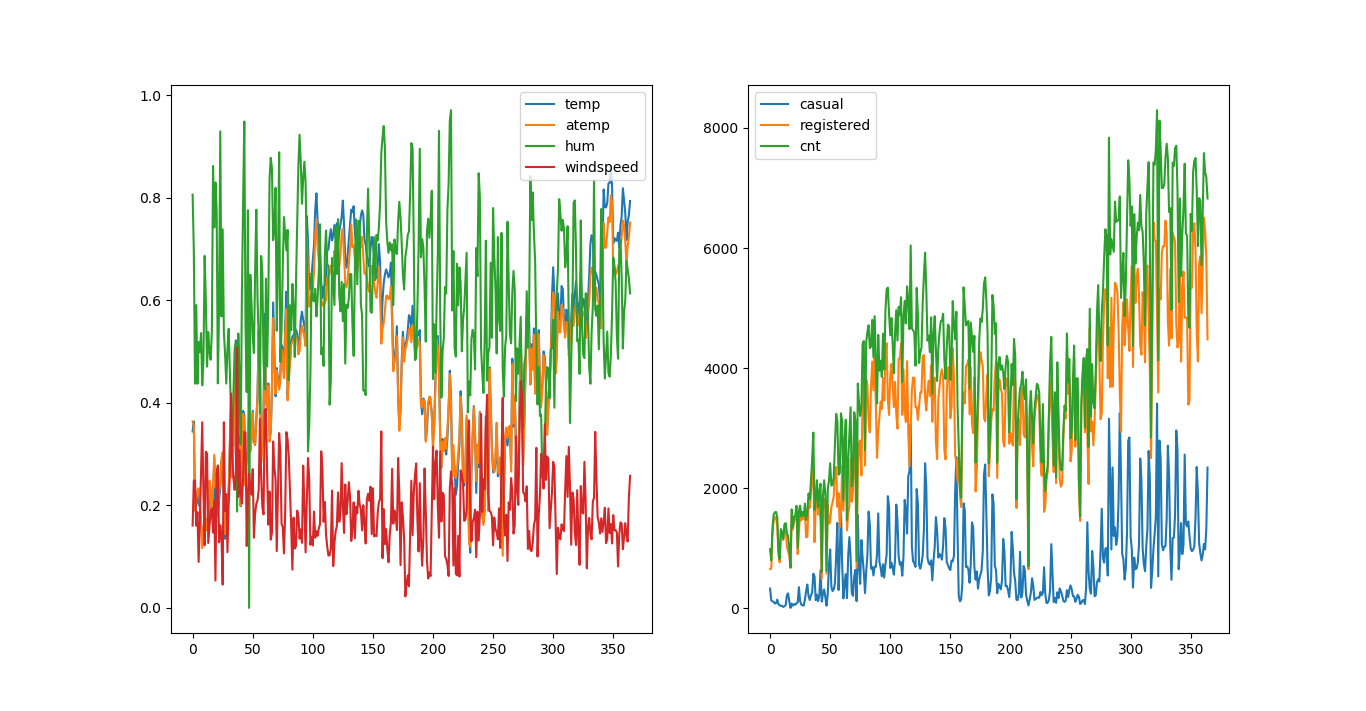
\includegraphics[width=.9\textwidth]{train-day}} \\
    \cprotect\subcaptionbox{\verbbox[gray]{hour.csv}训练集数据可视化\label{F:train-hour}}
        {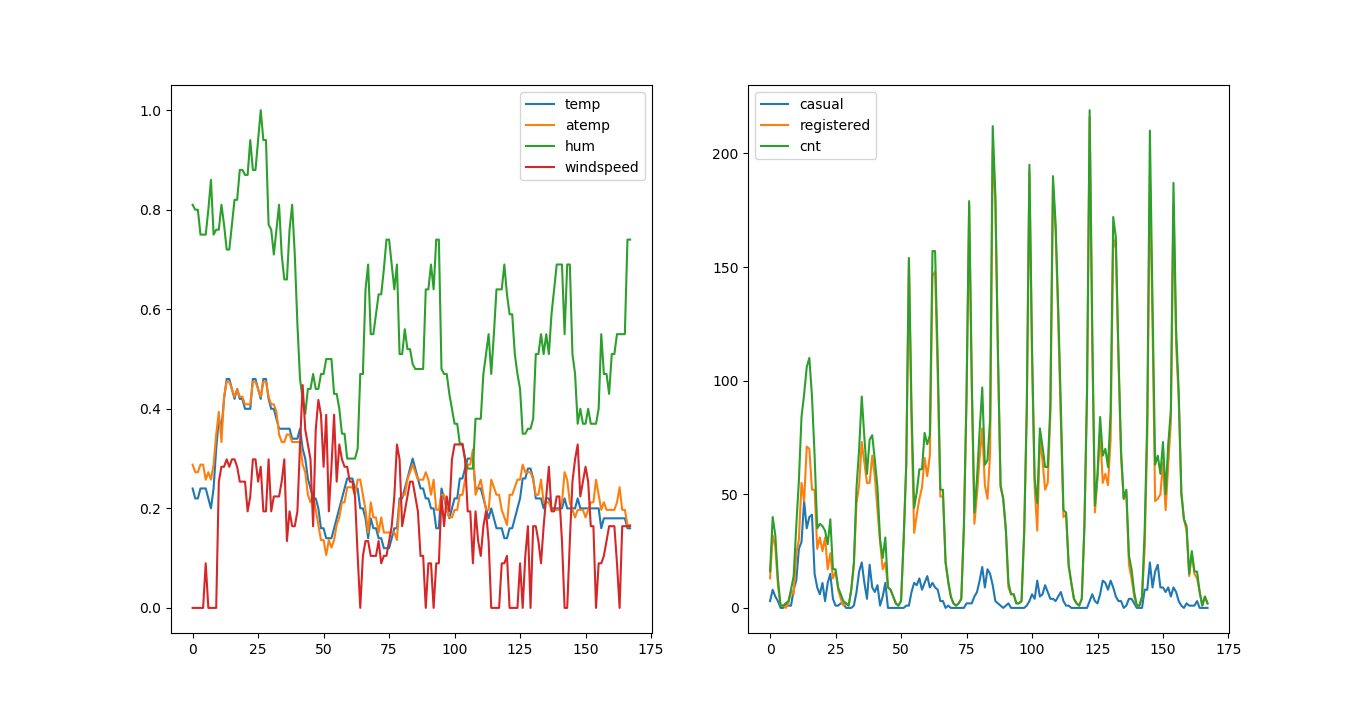
\includegraphics[width=.9\textwidth]{train-hour}}
    \caption{训练集数据可视化}\label{F:train}
\end{figure}

如图~\ref{F:test-day}与图~\ref{F:test-hour}可知,按照天数来说,用户数量的趋势与温度较为类似,而在小时尺度下则呈现不出明显的规律,有待于进一步的研究与建模。
\begin{figure}[htbp]
    \centering
    \cprotect\subcaptionbox{\verbbox[gray]{day.csv}测试集数据可视化\label{F:test-day}}
        {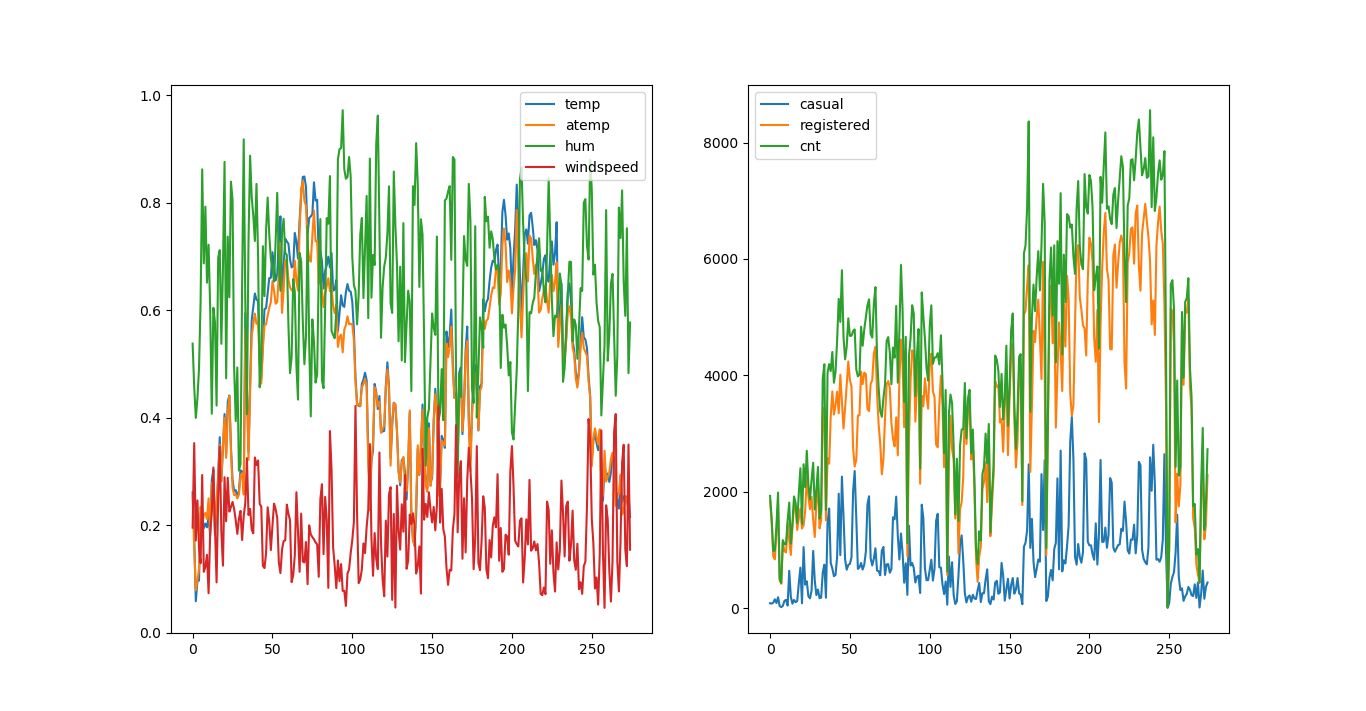
\includegraphics[width=.9\textwidth]{test-day}} \\
    \cprotect\subcaptionbox{\verbbox[gray]{hour.csv}测试集数据可视化\label{F:test-hour}}
        {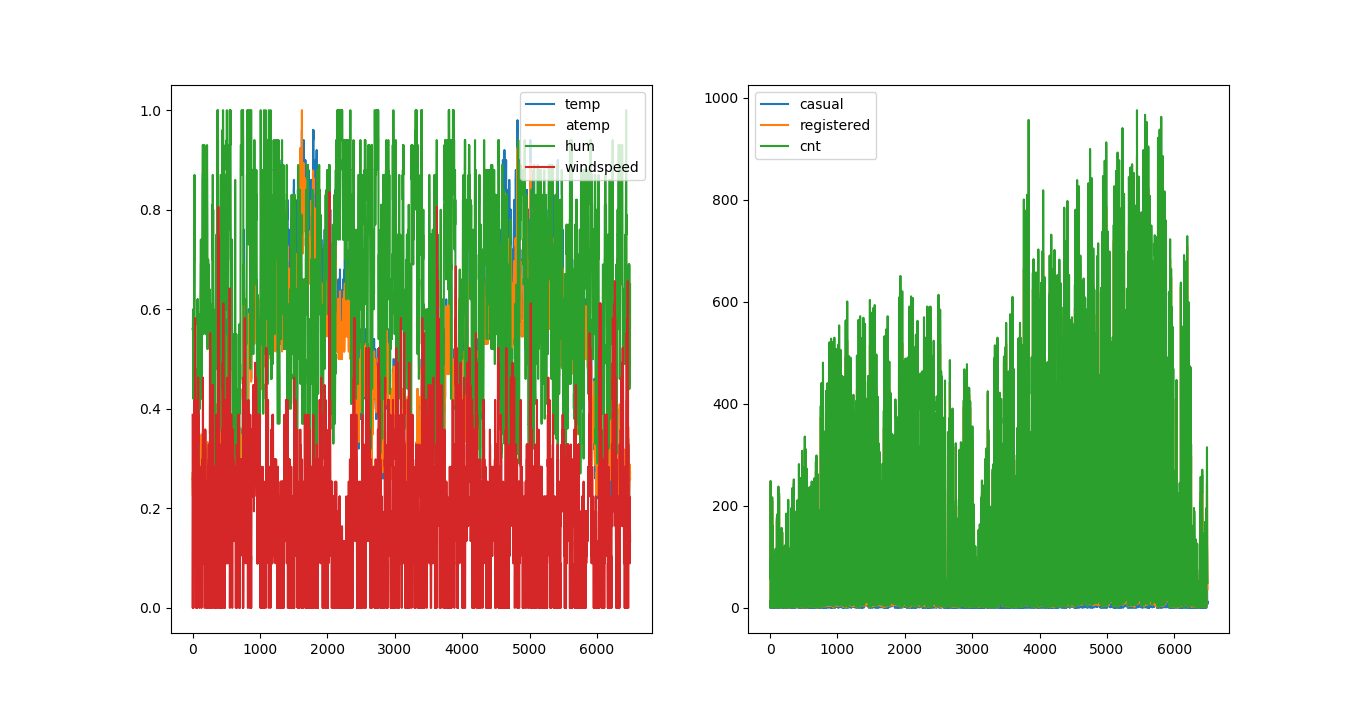
\includegraphics[width=.9\textwidth]{test-hour}}
    \caption{测试集数据可视化}\label{F:test}
\end{figure}

时间相关变量的训练集与测试集的数据趋势相差不大,因此我们只讨论训练集的数据可视化结果,如图~\ref{F:train-time}。

由图~\ref{F:train-time-hr}可知,不同颜色的线条对应着不同的时间点,而图中颜色呈现分层的效果,所以说用户数量与时间点之间存在较强的相关性。由图~\ref{F:train-time-mnth}与图~\ref{F:train-time-season}可知,2011年与2012年的数据呈现相似性,即大体趋势基本一致而对应月份的用户数量大致呈现倍数增加的关系。同时夏秋季节的用户数量多于春冬季节,符合温度对用户数量存在影响的假设。最后由图~\ref{F:train-time-workingday}可知,用户数量多的时间绝大部分为工作日,只有少数几天例外。
\begin{figure}[htbp]
    \centering
    \subcaptionbox{训练集上小时数与响应的关系图\label{F:train-time-hr}}
        {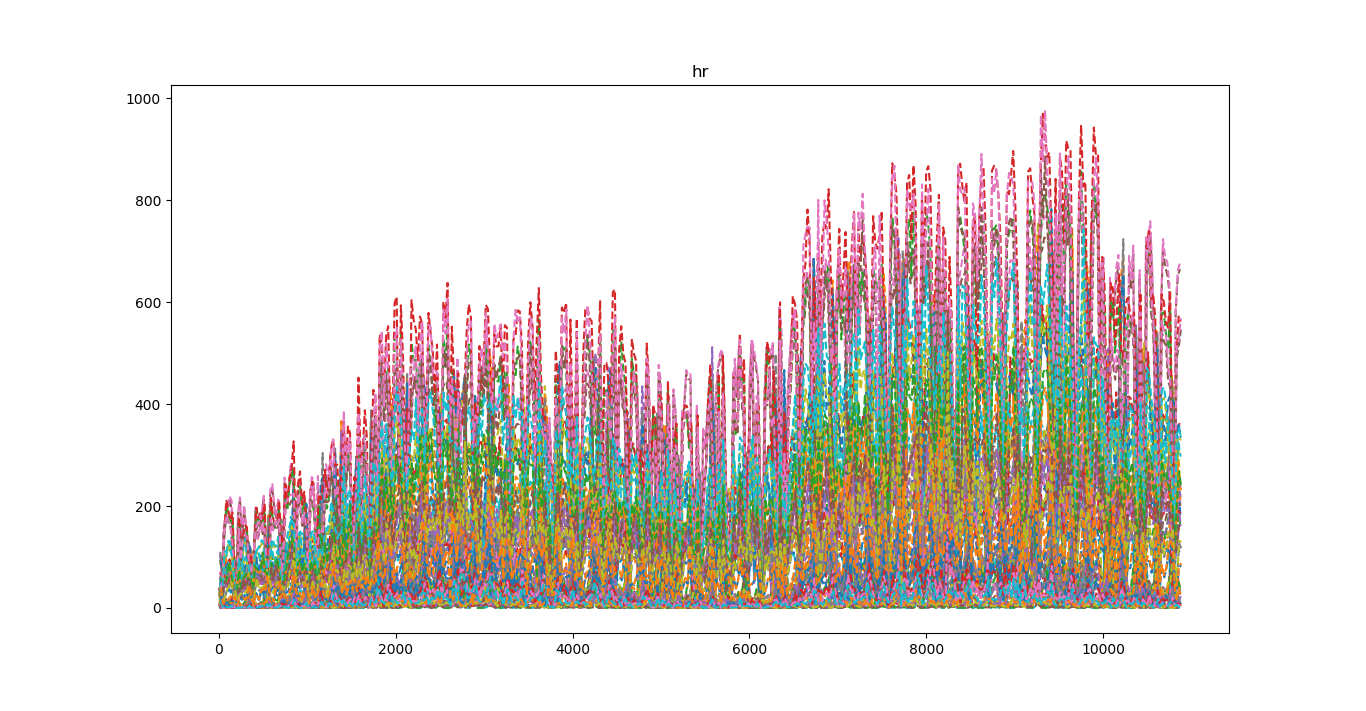
\includegraphics[width=.45\textwidth]{train-time-hr}}
    \subcaptionbox{训练集上月份与响应的关系图\label{F:train-time-mnth}}
        {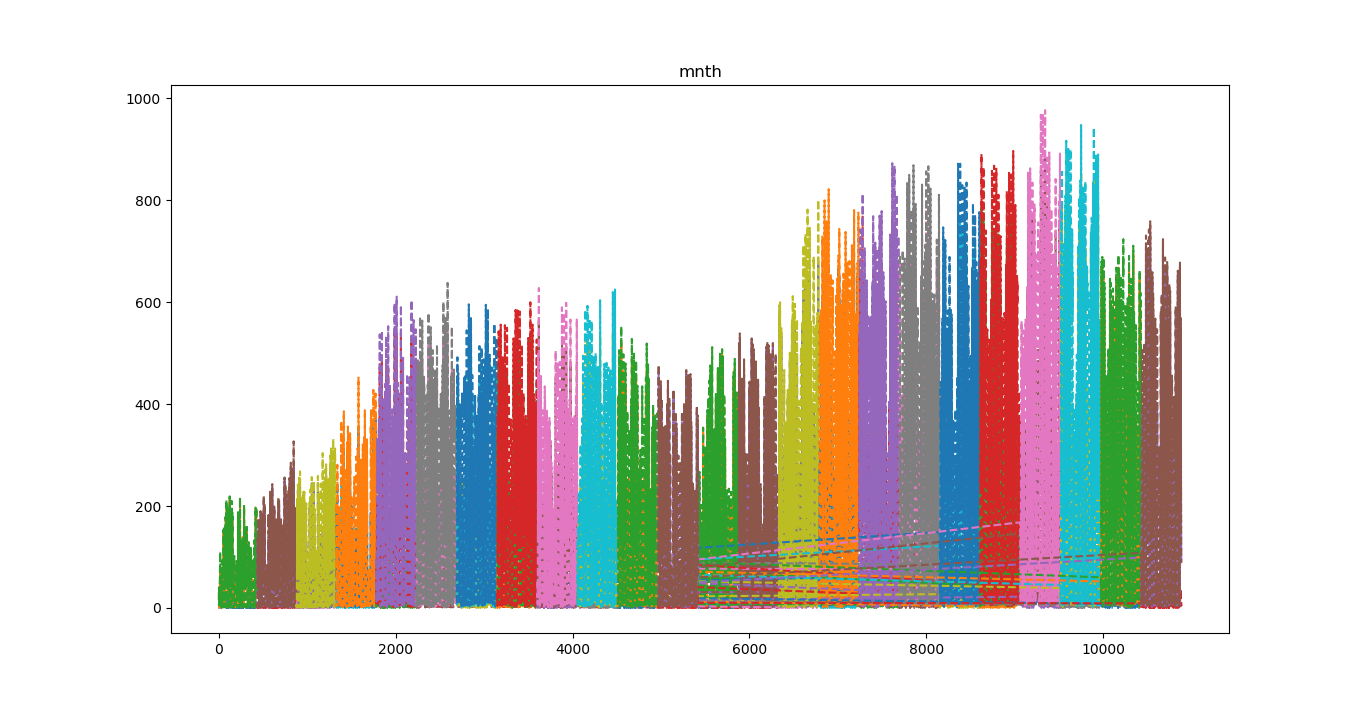
\includegraphics[width=.45\textwidth]{train-time-mnth}} \\
    \subcaptionbox{训练集上季节与响应的关系图\label{F:train-time-season}}
        {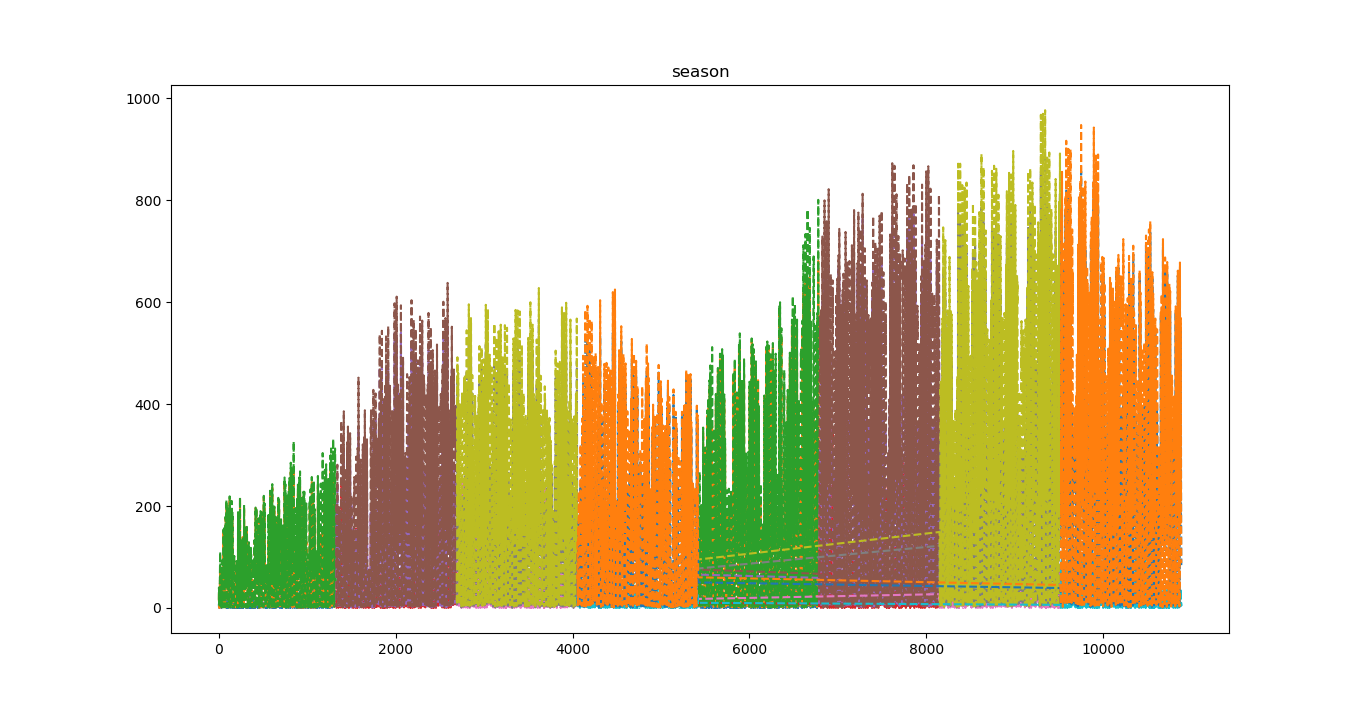
\includegraphics[width=.45\textwidth]{train-time-season}}
    \subcaptionbox{训练集上工作日与响应的关系图\label{F:train-time-workingday}}
        {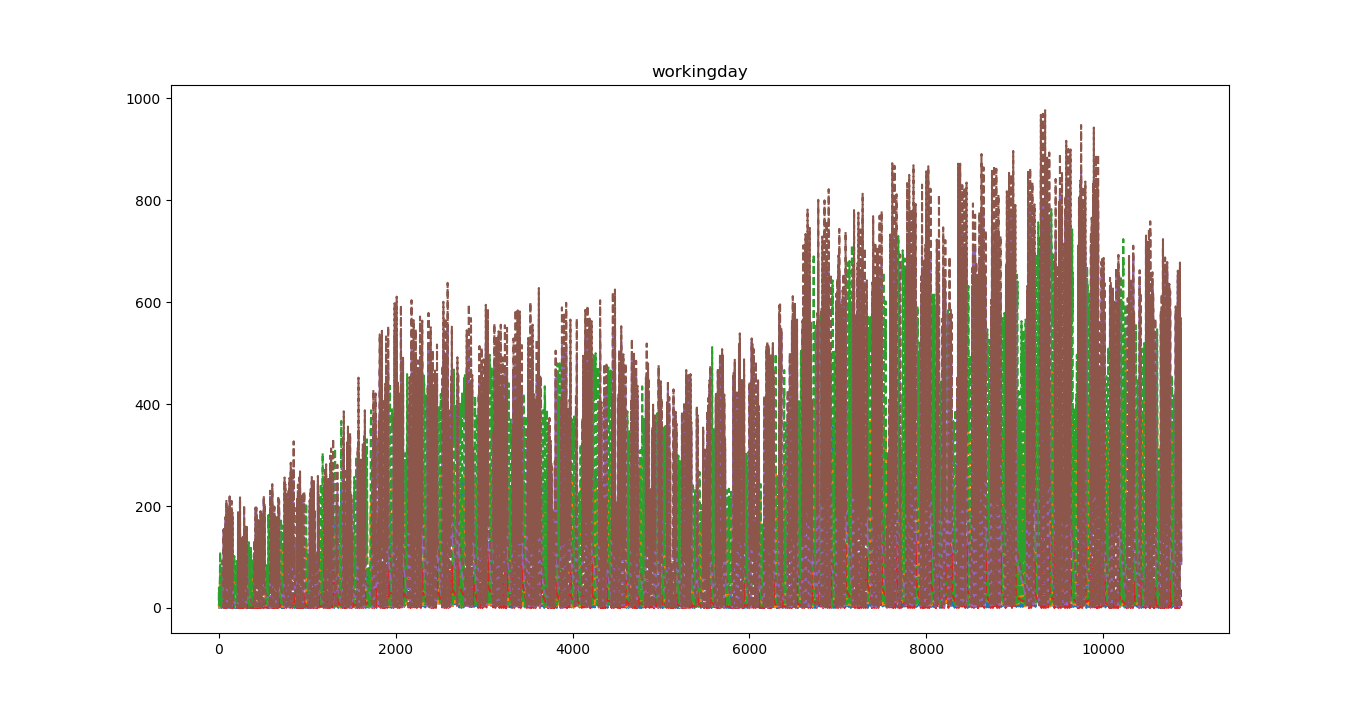
\includegraphics[width=.45\textwidth]{train-time-workingday}}
    \caption{训练集上时间有关变量与响应的关系图}\label{F:train-time}
\end{figure}

\begin{figure}[htbp]
    \centering
    \subcaptionbox{测试集上小时数与响应的关系图\label{F:test-time-hr}}
        {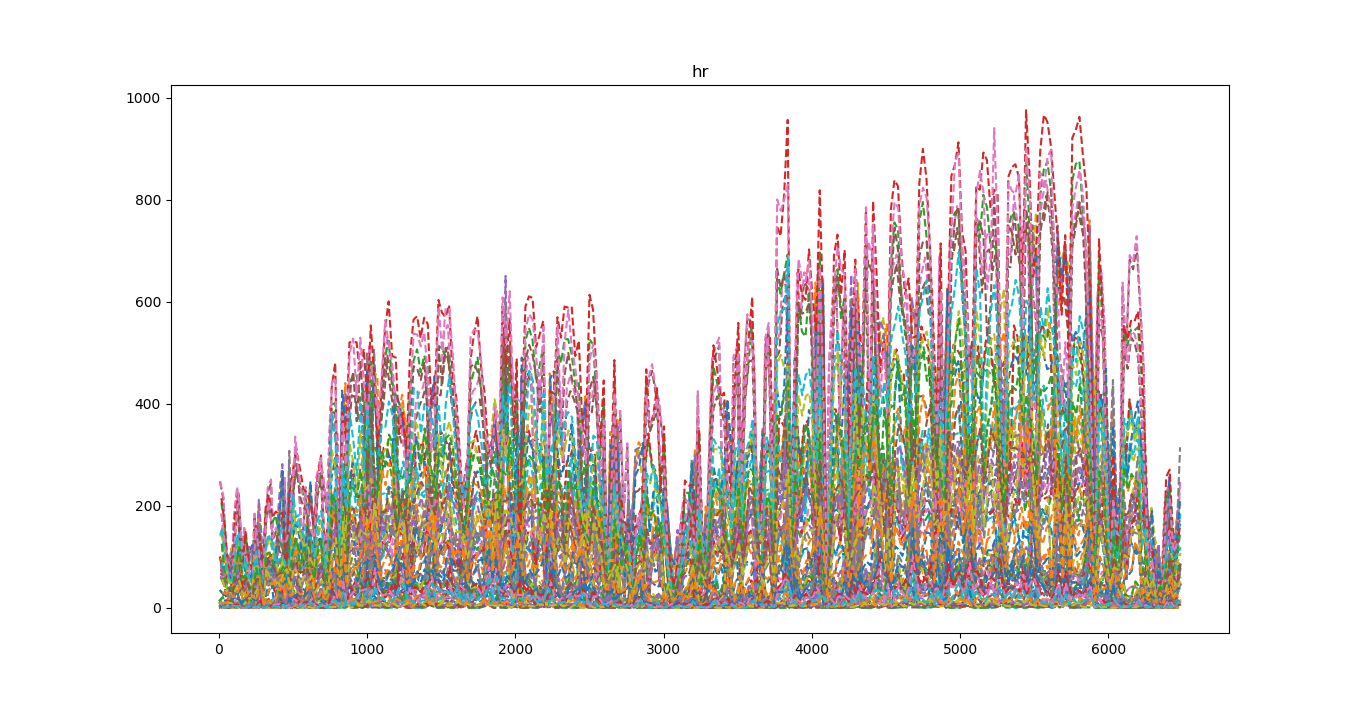
\includegraphics[width=.45\textwidth]{test-time-hr}}
    \subcaptionbox{测试集上月份与响应的关系图\label{F:test-time-mnth}}
        {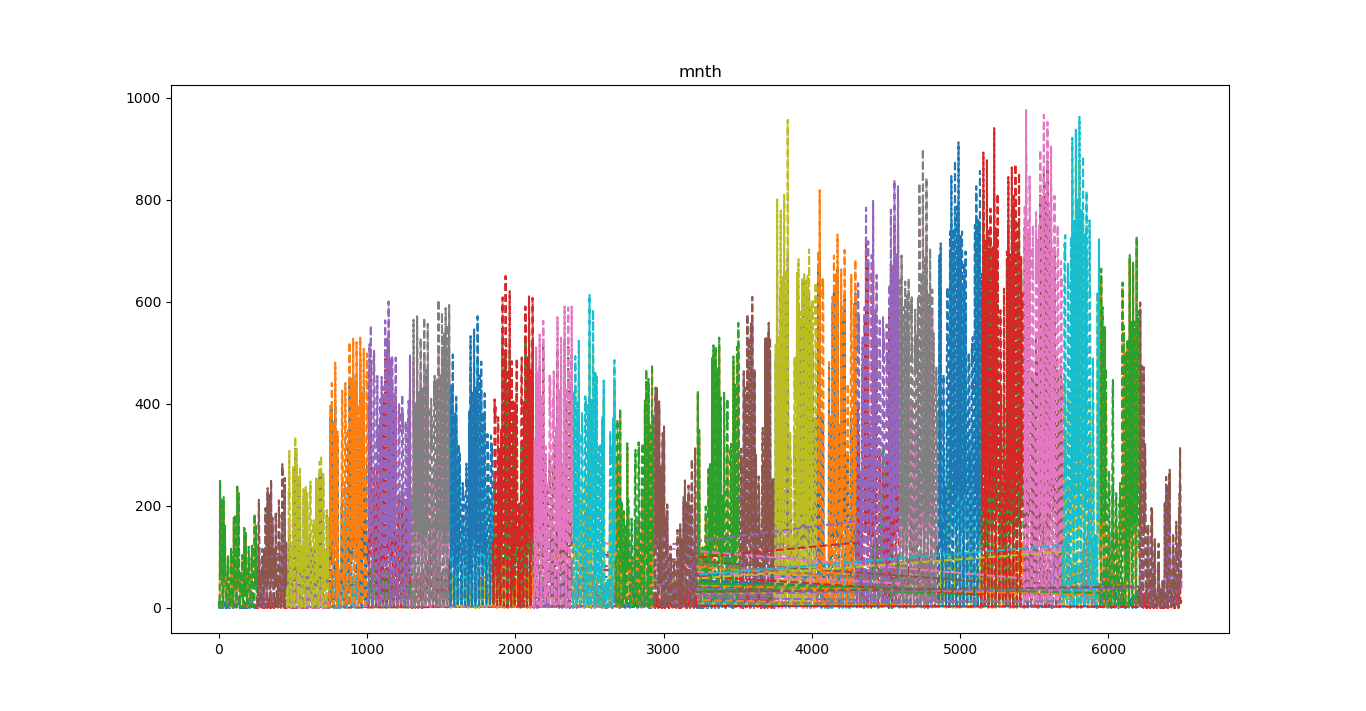
\includegraphics[width=.45\textwidth]{test-time-mnth}} \\
    \subcaptionbox{测试集上季节与响应的关系图\label{F:test-time-season}}
        {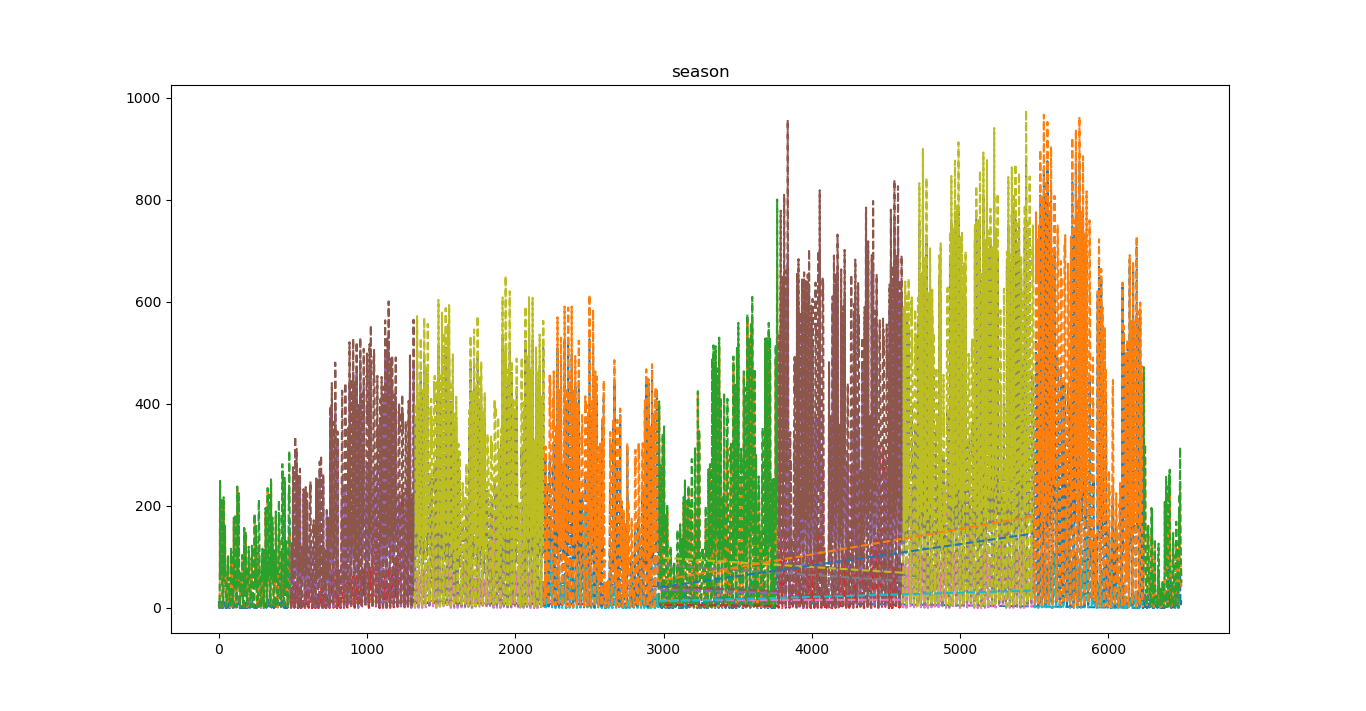
\includegraphics[width=.45\textwidth]{test-time-season}}
    \subcaptionbox{测试集上工作日与响应的关系图\label{F:test-time-workingday}}
        {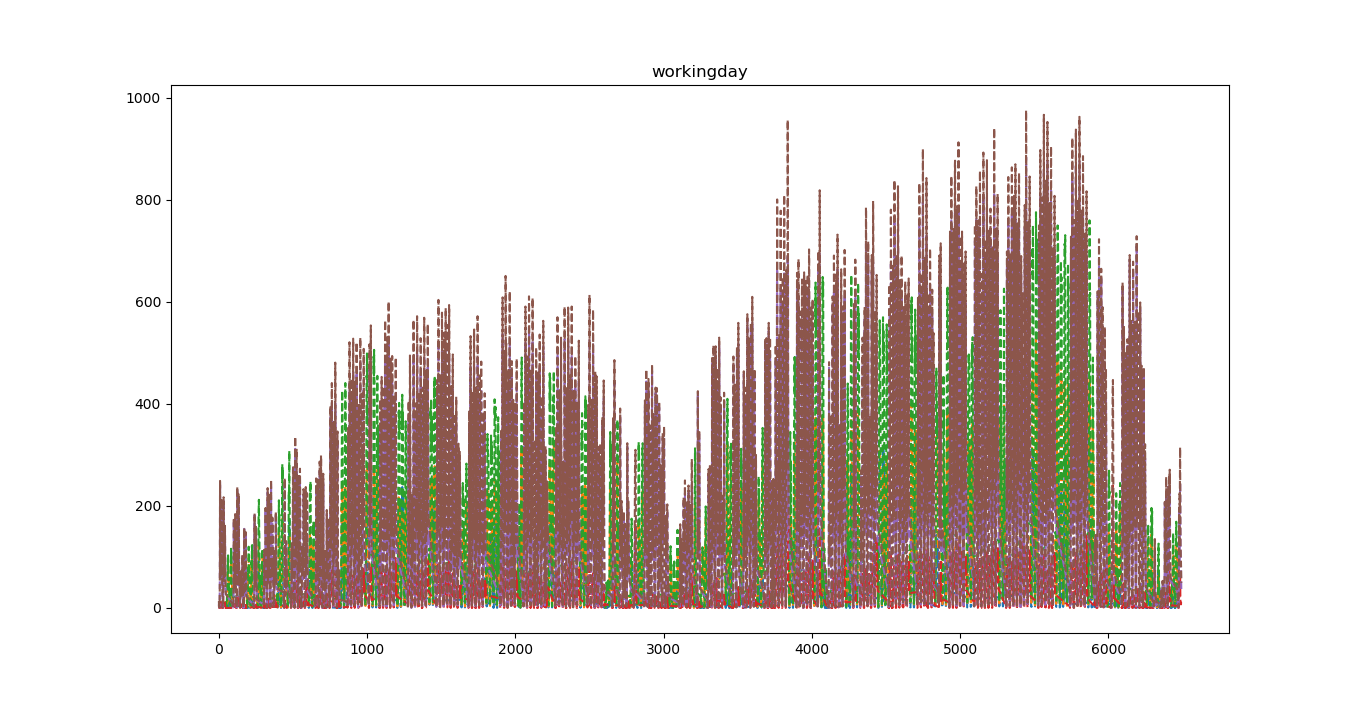
\includegraphics[width=.45\textwidth]{test-time-workingday}}
    \caption{测试集上时间有关变量与响应的关系图}\label{F:test-time}
\end{figure}
